\documentclass{standalone}
\usepackage{tikz}
\usetikzlibrary{patterns, positioning}

\begin{document}
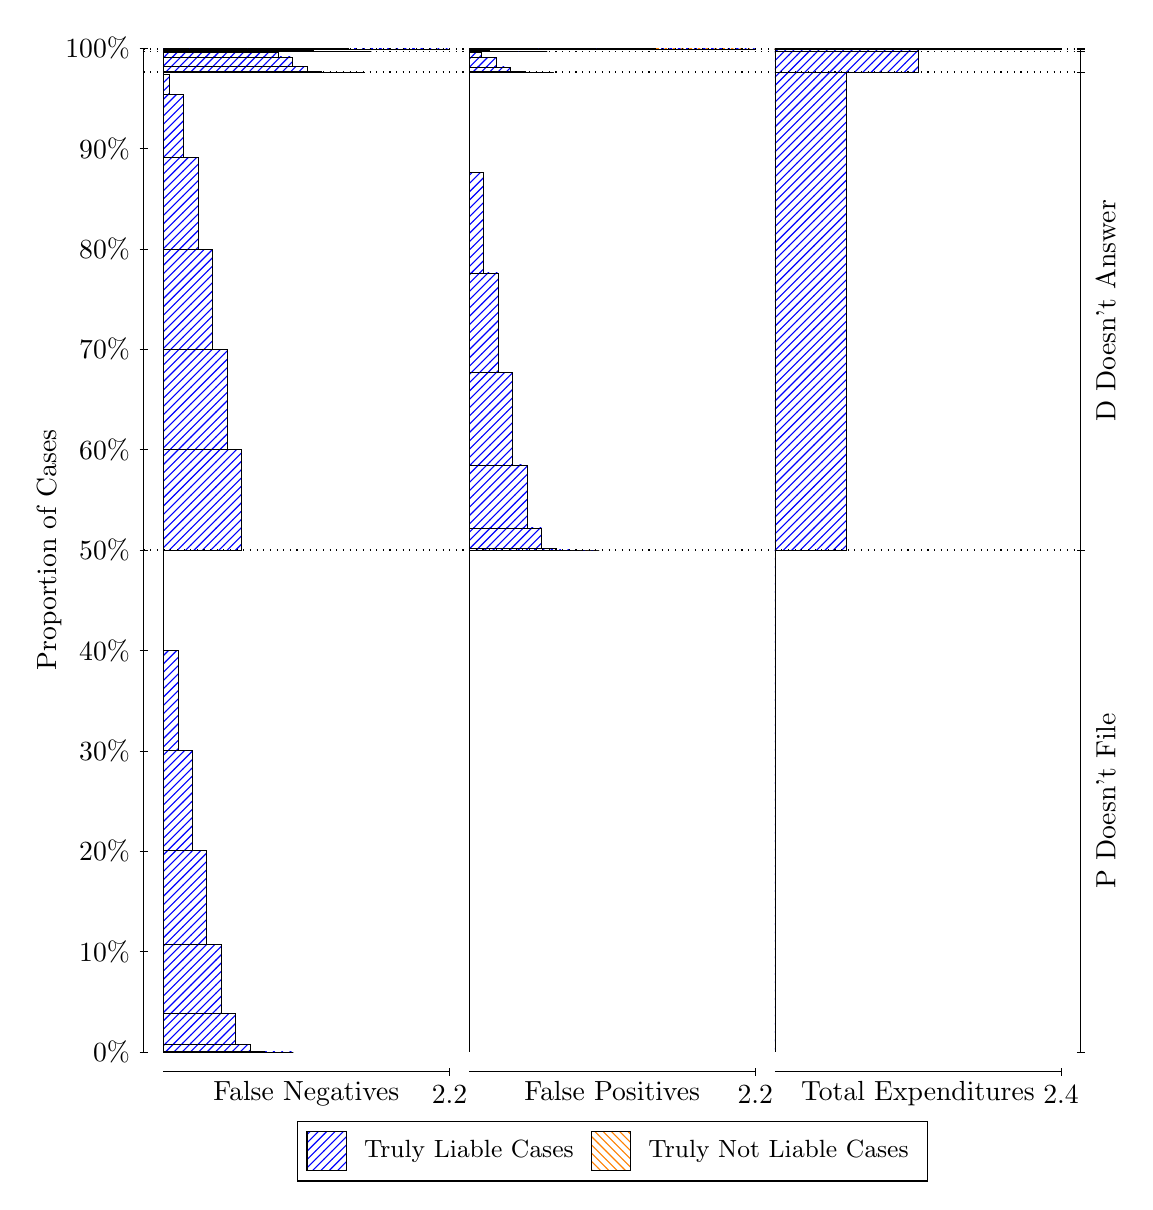
\begin{tikzpicture}
\draw[black, very thin] (1.5,1.75) -- (1.5,14.5);
\node[rotate=90, anchor=center] at (0.3, 8.125) {Proportion of Cases};
\draw[black, very thin] (1.45,1.75) -- (1.55,1.75);
\node[anchor=east] at (1.45, 1.75) {0\%};
\draw[black, very thin] (1.45,3.025) -- (1.55,3.025);
\node[anchor=east] at (1.45, 3.025) {10\%};
\draw[black, very thin] (1.45,4.3) -- (1.55,4.3);
\node[anchor=east] at (1.45, 4.3) {20\%};
\draw[black, very thin] (1.45,5.575) -- (1.55,5.575);
\node[anchor=east] at (1.45, 5.575) {30\%};
\draw[black, very thin] (1.45,6.85) -- (1.55,6.85);
\node[anchor=east] at (1.45, 6.85) {40\%};
\draw[black, very thin] (1.45,8.125) -- (1.55,8.125);
\node[anchor=east] at (1.45, 8.125) {50\%};
\draw[black, very thin] (1.45,9.4) -- (1.55,9.4);
\node[anchor=east] at (1.45, 9.4) {60\%};
\draw[black, very thin] (1.45,10.675) -- (1.55,10.675);
\node[anchor=east] at (1.45, 10.675) {70\%};
\draw[black, very thin] (1.45,11.95) -- (1.55,11.95);
\node[anchor=east] at (1.45, 11.95) {80\%};
\draw[black, very thin] (1.45,13.225) -- (1.55,13.225);
\node[anchor=east] at (1.45, 13.225) {90\%};
\draw[black, very thin] (1.45,14.5) -- (1.55,14.5);
\node[anchor=east] at (1.45, 14.5) {100\%};

\draw[black, very thin] (13.4,1.75) -- (13.4,14.5);
\draw[black, very thin] (13.35,1.75) -- (13.45,1.75);
\node[anchor=west] at (13.35, 1.75) {};
\draw[black, very thin] (13.35,8.125) -- (13.45,8.125);
\node[anchor=west] at (13.35, 8.125) {};
\draw[black, very thin] (13.35,14.195) -- (13.45,14.195);
\node[anchor=west] at (13.35, 14.195) {};
\draw[black, very thin] (13.35,14.453) -- (13.45,14.453);
\node[anchor=west] at (13.35, 14.453) {};
\draw[black, very thin] (13.35,14.48) -- (13.45,14.48);
\node[anchor=west] at (13.35, 14.48) {};
\draw[black, very thin] (13.35,14.489) -- (13.45,14.489);
\node[anchor=west] at (13.35, 14.489) {};
\draw[black, very thin] (13.35,14.5) -- (13.45,14.5);
\node[anchor=west] at (13.35, 14.5) {};

\draw[black, very thin, pattern color=blue, pattern=north east lines] (1.75,1.75) rectangle (3.4015,1.75);
\draw[black, very thin, pattern color=blue, pattern=north east lines] (1.75,1.75) rectangle (3.218,1.7503);
\draw[black, very thin, pattern color=blue, pattern=north east lines] (1.75,1.7503) rectangle (3.0345,1.7583);
\draw[black, very thin, pattern color=blue, pattern=north east lines] (1.75,1.7583) rectangle (2.851,1.8435);
\draw[black, very thin, pattern color=blue, pattern=north east lines] (1.75,1.8435) rectangle (2.6675,2.2369);
\draw[black, very thin, pattern color=blue, pattern=north east lines] (1.75,2.2369) rectangle (2.484,3.1185);
\draw[black, very thin, pattern color=blue, pattern=north east lines] (1.75,3.1185) rectangle (2.3005,4.3083);
\draw[black, very thin, pattern color=blue, pattern=north east lines] (1.75,4.3083) rectangle (2.117,5.5753);
\draw[black, very thin, pattern color=blue, pattern=north east lines] (1.75,5.5753) rectangle (1.9335,6.85);
\draw[black, very thin, pattern color=orange, pattern=north west lines] (1.75,6.85) rectangle (1.75,6.85);
\draw[black, very thin, pattern color=blue, pattern=north east lines] (1.75,6.85) rectangle (1.75,8.125);
\draw[black, very thin, pattern color=blue, pattern=north east lines] (1.75,8.125) rectangle (2.7409,9.4);
\draw[black, very thin, pattern color=blue, pattern=north east lines] (1.75,9.4) rectangle (2.5574,10.675);
\draw[black, very thin, pattern color=blue, pattern=north east lines] (1.75,10.675) rectangle (2.3739,11.941);
\draw[black, very thin, pattern color=blue, pattern=north east lines] (1.75,11.941) rectangle (2.1904,13.115);
\draw[black, very thin, pattern color=blue, pattern=north east lines] (1.75,13.115) rectangle (2.0069,13.915);
\draw[black, very thin, pattern color=blue, pattern=north east lines] (1.75,13.915) rectangle (1.8234,14.17);
\draw[black, very thin, pattern color=orange, pattern=north west lines] (1.75,14.17) rectangle (1.75,14.17);
\draw[black, very thin, pattern color=blue, pattern=north east lines] (1.75,14.17) rectangle (1.75,14.195);
\draw[black, very thin, pattern color=blue, pattern=north east lines] (1.75,14.195) rectangle (4.3098,14.195);
\draw[black, very thin, pattern color=blue, pattern=north east lines] (1.75,14.195) rectangle (4.1263,14.195);
\draw[black, very thin, pattern color=blue, pattern=north east lines] (1.75,14.195) rectangle (3.9428,14.195);
\draw[black, very thin, pattern color=blue, pattern=north east lines] (1.75,14.195) rectangle (3.7593,14.202);
\draw[black, very thin, pattern color=blue, pattern=north east lines] (1.75,14.202) rectangle (3.5758,14.264);
\draw[black, very thin, pattern color=blue, pattern=north east lines] (1.75,14.264) rectangle (3.3923,14.387);
\draw[black, very thin, pattern color=blue, pattern=north east lines] (1.75,14.387) rectangle (3.2088,14.446);
\draw[black, very thin, pattern color=blue, pattern=north east lines] (1.75,14.446) rectangle (3.0253,14.453);
\draw[black, very thin, pattern color=blue, pattern=north east lines] (1.75,14.453) rectangle (2.8418,14.453);
\draw[black, very thin, pattern color=blue, pattern=north east lines] (1.75,14.453) rectangle (2.6583,14.453);
\draw[black, very thin, pattern color=orange, pattern=north west lines] (1.75,14.453) rectangle (1.75,14.453);
\draw[black, very thin, pattern color=blue, pattern=north east lines] (1.75,14.453) rectangle (4.3924,14.453);
\draw[black, very thin, pattern color=blue, pattern=north east lines] (1.75,14.453) rectangle (4.2089,14.453);
\draw[black, very thin, pattern color=blue, pattern=north east lines] (1.75,14.453) rectangle (4.0254,14.453);
\draw[black, very thin, pattern color=blue, pattern=north east lines] (1.75,14.453) rectangle (3.8419,14.455);
\draw[black, very thin, pattern color=blue, pattern=north east lines] (1.75,14.455) rectangle (3.6584,14.466);
\draw[black, very thin, pattern color=blue, pattern=north east lines] (1.75,14.466) rectangle (3.4749,14.477);
\draw[black, very thin, pattern color=blue, pattern=north east lines] (1.75,14.477) rectangle (3.2914,14.48);
\draw[black, very thin, pattern color=blue, pattern=north east lines] (1.75,14.48) rectangle (3.1079,14.48);
\draw[black, very thin, pattern color=blue, pattern=north east lines] (1.75,14.48) rectangle (2.9244,14.48);
\draw[black, very thin, pattern color=blue, pattern=north east lines] (1.75,14.48) rectangle (2.7409,14.48);
\draw[black, very thin, pattern color=orange, pattern=north west lines] (1.75,14.48) rectangle (1.75,14.48);
\draw[black, very thin, pattern color=blue, pattern=north east lines] (1.75,14.48) rectangle (2.7409,14.48);
\draw[black, very thin, pattern color=blue, pattern=north east lines] (1.75,14.48) rectangle (2.5574,14.48);
\draw[black, very thin, pattern color=blue, pattern=north east lines] (1.75,14.48) rectangle (2.3739,14.481);
\draw[black, very thin, pattern color=blue, pattern=north east lines] (1.75,14.481) rectangle (2.1904,14.484);
\draw[black, very thin, pattern color=blue, pattern=north east lines] (1.75,14.484) rectangle (2.0069,14.488);
\draw[black, very thin, pattern color=blue, pattern=north east lines] (1.75,14.488) rectangle (1.8234,14.489);
\draw[black, very thin, pattern color=orange, pattern=north west lines] (1.75,14.489) rectangle (1.75,14.489);
\draw[black, very thin, pattern color=blue, pattern=north east lines] (1.75,14.489) rectangle (1.75,14.489);
\draw[black, very thin, pattern color=blue, pattern=north east lines] (1.75,14.489) rectangle (5.3833,14.489);
\draw[black, very thin, pattern color=blue, pattern=north east lines] (1.75,14.489) rectangle (5.1998,14.489);
\draw[black, very thin, pattern color=blue, pattern=north east lines] (1.75,14.489) rectangle (5.0163,14.489);
\draw[black, very thin, pattern color=blue, pattern=north east lines] (1.75,14.489) rectangle (5.0163,14.489);
\draw[black, very thin, pattern color=blue, pattern=north east lines] (1.75,14.489) rectangle (4.8328,14.489);
\draw[black, very thin, pattern color=blue, pattern=north east lines] (1.75,14.489) rectangle (4.6493,14.489);
\draw[black, very thin, pattern color=blue, pattern=north east lines] (1.75,14.489) rectangle (4.4658,14.489);
\draw[black, very thin, pattern color=blue, pattern=north east lines] (1.75,14.489) rectangle (4.2823,14.49);
\draw[black, very thin, pattern color=blue, pattern=north east lines] (1.75,14.49) rectangle (4.0988,14.49);
\draw[black, very thin, pattern color=blue, pattern=north east lines] (1.75,14.49) rectangle (4.0988,14.491);
\draw[black, very thin, pattern color=blue, pattern=north east lines] (1.75,14.491) rectangle (3.9153,14.493);
\draw[black, very thin, pattern color=blue, pattern=north east lines] (1.75,14.493) rectangle (3.9153,14.493);
\draw[black, very thin, pattern color=blue, pattern=north east lines] (1.75,14.493) rectangle (3.7318,14.496);
\draw[black, very thin, pattern color=blue, pattern=north east lines] (1.75,14.496) rectangle (3.5483,14.497);
\draw[black, very thin, pattern color=blue, pattern=north east lines] (1.75,14.497) rectangle (3.5483,14.498);
\draw[black, very thin, pattern color=blue, pattern=north east lines] (1.75,14.498) rectangle (3.3648,14.498);
\draw[black, very thin, pattern color=blue, pattern=north east lines] (1.75,14.498) rectangle (3.3648,14.499);
\draw[black, very thin, pattern color=blue, pattern=north east lines] (1.75,14.499) rectangle (3.3648,14.5);
\draw[black, very thin, pattern color=blue, pattern=north east lines] (1.75,14.5) rectangle (3.1813,14.5);
\draw[black, very thin, pattern color=blue, pattern=north east lines] (1.75,14.5) rectangle (3.1813,14.5);
\draw[black, very thin, pattern color=blue, pattern=north east lines] (1.75,14.5) rectangle (2.9978,14.5);
\draw[black, very thin, pattern color=blue, pattern=north east lines] (1.75,14.5) rectangle (2.8143,14.5);
\draw[black, very thin, pattern color=blue, pattern=north east lines] (1.75,14.5) rectangle (2.6308,14.5);
\draw[black, very thin, pattern color=blue, pattern=north east lines] (1.75,14.5) rectangle (2.6308,14.5);
\draw[black, very thin, pattern color=blue, pattern=north east lines] (1.75,14.5) rectangle (2.4473,14.5);
\draw[black, very thin, pattern color=blue, pattern=north east lines] (1.75,14.5) rectangle (2.4473,14.5);
\draw[black, very thin, pattern color=blue, pattern=north east lines] (1.75,14.5) rectangle (2.2638,14.5);
\draw[black, very thin, pattern color=blue, pattern=north east lines] (1.75,14.5) rectangle (2.2638,14.5);
\draw[black, very thin, pattern color=blue, pattern=north east lines] (1.75,14.5) rectangle (2.0803,14.5);
\draw[black, very thin, pattern color=orange, pattern=north west lines] (1.75,14.5) rectangle (1.75,14.5);
\draw[black, very thin, pattern color=orange, pattern=north west lines] (5.6333,1.75) rectangle (5.6333,1.75);
\draw[black, very thin, pattern color=blue, pattern=north east lines] (5.6333,1.75) rectangle (5.6333,8.125);
\draw[black, very thin, pattern color=orange, pattern=north west lines] (5.6333,8.125) rectangle (7.2848,8.125);
\draw[black, very thin, pattern color=blue, pattern=north east lines] (5.6333,8.125) rectangle (7.2848,8.125);
\draw[black, very thin, pattern color=blue, pattern=north east lines] (5.6333,8.125) rectangle (7.1013,8.125);
\draw[black, very thin, pattern color=blue, pattern=north east lines] (5.6333,8.125) rectangle (6.9178,8.1255);
\draw[black, very thin, pattern color=blue, pattern=north east lines] (5.6333,8.1255) rectangle (6.7343,8.1495);
\draw[black, very thin, pattern color=blue, pattern=north east lines] (5.6333,8.1495) rectangle (6.5508,8.4051);
\draw[black, very thin, pattern color=blue, pattern=north east lines] (5.6333,8.4051) rectangle (6.3673,9.2046);
\draw[black, very thin, pattern color=blue, pattern=north east lines] (5.6333,9.2046) rectangle (6.1838,10.379);
\draw[black, very thin, pattern color=blue, pattern=north east lines] (5.6333,10.379) rectangle (6.0003,11.645);
\draw[black, very thin, pattern color=blue, pattern=north east lines] (5.6333,11.645) rectangle (5.8168,12.92);
\draw[black, very thin, pattern color=blue, pattern=north east lines] (5.6333,12.92) rectangle (5.6333,14.195);
\draw[black, very thin, pattern color=orange, pattern=north west lines] (5.6333,14.195) rectangle (6.7068,14.195);
\draw[black, very thin, pattern color=blue, pattern=north east lines] (5.6333,14.195) rectangle (6.7068,14.195);
\draw[black, very thin, pattern color=blue, pattern=north east lines] (5.6333,14.195) rectangle (6.5233,14.195);
\draw[black, very thin, pattern color=blue, pattern=north east lines] (5.6333,14.195) rectangle (6.3398,14.202);
\draw[black, very thin, pattern color=blue, pattern=north east lines] (5.6333,14.202) rectangle (6.1563,14.261);
\draw[black, very thin, pattern color=blue, pattern=north east lines] (5.6333,14.261) rectangle (5.9728,14.384);
\draw[black, very thin, pattern color=blue, pattern=north east lines] (5.6333,14.384) rectangle (5.7893,14.446);
\draw[black, very thin, pattern color=blue, pattern=north east lines] (5.6333,14.446) rectangle (5.6333,14.453);
\draw[black, very thin, pattern color=orange, pattern=north west lines] (5.6333,14.453) rectangle (6.6242,14.453);
\draw[black, very thin, pattern color=blue, pattern=north east lines] (5.6333,14.453) rectangle (6.6242,14.453);
\draw[black, very thin, pattern color=blue, pattern=north east lines] (5.6333,14.453) rectangle (6.4407,14.453);
\draw[black, very thin, pattern color=blue, pattern=north east lines] (5.6333,14.453) rectangle (6.2572,14.453);
\draw[black, very thin, pattern color=blue, pattern=north east lines] (5.6333,14.453) rectangle (6.0737,14.456);
\draw[black, very thin, pattern color=blue, pattern=north east lines] (5.6333,14.456) rectangle (5.8902,14.467);
\draw[black, very thin, pattern color=blue, pattern=north east lines] (5.6333,14.467) rectangle (5.7067,14.478);
\draw[black, very thin, pattern color=blue, pattern=north east lines] (5.6333,14.478) rectangle (5.6333,14.48);
\draw[black, very thin, pattern color=orange, pattern=north west lines] (5.6333,14.48) rectangle (8.2758,14.48);
\draw[black, very thin, pattern color=blue, pattern=north east lines] (5.6333,14.48) rectangle (8.2758,14.48);
\draw[black, very thin, pattern color=blue, pattern=north east lines] (5.6333,14.48) rectangle (8.0923,14.48);
\draw[black, very thin, pattern color=blue, pattern=north east lines] (5.6333,14.48) rectangle (7.9088,14.48);
\draw[black, very thin, pattern color=blue, pattern=north east lines] (5.6333,14.48) rectangle (7.7253,14.48);
\draw[black, very thin, pattern color=blue, pattern=north east lines] (5.6333,14.48) rectangle (7.5418,14.481);
\draw[black, very thin, pattern color=blue, pattern=north east lines] (5.6333,14.481) rectangle (7.3582,14.485);
\draw[black, very thin, pattern color=blue, pattern=north east lines] (5.6333,14.485) rectangle (7.1747,14.488);
\draw[black, very thin, pattern color=blue, pattern=north east lines] (5.6333,14.488) rectangle (6.9912,14.489);
\draw[black, very thin, pattern color=blue, pattern=north east lines] (5.6333,14.489) rectangle (6.8077,14.489);
\draw[black, very thin, pattern color=blue, pattern=north east lines] (5.6333,14.489) rectangle (6.6242,14.489);
\draw[black, very thin, pattern color=orange, pattern=north west lines] (5.6333,14.489) rectangle (9.2667,14.489);
\draw[black, very thin, pattern color=blue, pattern=north east lines] (5.6333,14.489) rectangle (9.2667,14.489);
\draw[black, very thin, pattern color=blue, pattern=north east lines] (5.6333,14.489) rectangle (9.0832,14.489);
\draw[black, very thin, pattern color=orange, pattern=north west lines] (5.6333,14.489) rectangle (9.0832,14.489);
\draw[black, very thin, pattern color=blue, pattern=north east lines] (5.6333,14.489) rectangle (9.0832,14.489);
\draw[black, very thin, pattern color=orange, pattern=north west lines] (5.6333,14.489) rectangle (8.8997,14.489);
\draw[black, very thin, pattern color=blue, pattern=north east lines] (5.6333,14.489) rectangle (8.8997,14.489);
\draw[black, very thin, pattern color=blue, pattern=north east lines] (5.6333,14.489) rectangle (8.8997,14.489);
\draw[black, very thin, pattern color=blue, pattern=north east lines] (5.6333,14.489) rectangle (8.7162,14.489);
\draw[black, very thin, pattern color=orange, pattern=north west lines] (5.6333,14.489) rectangle (8.7162,14.489);
\draw[black, very thin, pattern color=blue, pattern=north east lines] (5.6333,14.489) rectangle (8.7162,14.489);
\draw[black, very thin, pattern color=blue, pattern=north east lines] (5.6333,14.489) rectangle (8.7162,14.489);
\draw[black, very thin, pattern color=blue, pattern=north east lines] (5.6333,14.489) rectangle (8.5327,14.489);
\draw[black, very thin, pattern color=orange, pattern=north west lines] (5.6333,14.489) rectangle (8.5327,14.489);
\draw[black, very thin, pattern color=blue, pattern=north east lines] (5.6333,14.489) rectangle (8.5327,14.489);
\draw[black, very thin, pattern color=blue, pattern=north east lines] (5.6333,14.489) rectangle (8.5327,14.489);
\draw[black, very thin, pattern color=blue, pattern=north east lines] (5.6333,14.489) rectangle (8.3492,14.489);
\draw[black, very thin, pattern color=orange, pattern=north west lines] (5.6333,14.489) rectangle (8.3492,14.489);
\draw[black, very thin, pattern color=blue, pattern=north east lines] (5.6333,14.489) rectangle (8.3492,14.489);
\draw[black, very thin, pattern color=blue, pattern=north east lines] (5.6333,14.489) rectangle (8.3492,14.489);
\draw[black, very thin, pattern color=blue, pattern=north east lines] (5.6333,14.489) rectangle (8.1657,14.489);
\draw[black, very thin, pattern color=blue, pattern=north east lines] (5.6333,14.489) rectangle (8.1657,14.489);
\draw[black, very thin, pattern color=orange, pattern=north west lines] (5.6333,14.489) rectangle (8.1657,14.489);
\draw[black, very thin, pattern color=blue, pattern=north east lines] (5.6333,14.489) rectangle (8.1657,14.489);
\draw[black, very thin, pattern color=blue, pattern=north east lines] (5.6333,14.489) rectangle (8.1657,14.49);
\draw[black, very thin, pattern color=blue, pattern=north east lines] (5.6333,14.49) rectangle (7.9822,14.49);
\draw[black, very thin, pattern color=blue, pattern=north east lines] (5.6333,14.49) rectangle (7.9822,14.49);
\draw[black, very thin, pattern color=orange, pattern=north west lines] (5.6333,14.49) rectangle (7.9822,14.49);
\draw[black, very thin, pattern color=blue, pattern=north east lines] (5.6333,14.49) rectangle (7.9822,14.491);
\draw[black, very thin, pattern color=blue, pattern=north east lines] (5.6333,14.491) rectangle (7.7987,14.491);
\draw[black, very thin, pattern color=orange, pattern=north west lines] (5.6333,14.491) rectangle (7.7987,14.491);
\draw[black, very thin, pattern color=blue, pattern=north east lines] (5.6333,14.491) rectangle (7.7987,14.493);
\draw[black, very thin, pattern color=blue, pattern=north east lines] (5.6333,14.493) rectangle (7.7987,14.493);
\draw[black, very thin, pattern color=blue, pattern=north east lines] (5.6333,14.493) rectangle (7.6152,14.494);
\draw[black, very thin, pattern color=orange, pattern=north west lines] (5.6333,14.494) rectangle (7.6152,14.494);
\draw[black, very thin, pattern color=blue, pattern=north east lines] (5.6333,14.494) rectangle (7.6152,14.496);
\draw[black, very thin, pattern color=blue, pattern=north east lines] (5.6333,14.496) rectangle (7.6152,14.496);
\draw[black, very thin, pattern color=blue, pattern=north east lines] (5.6333,14.496) rectangle (7.4316,14.496);
\draw[black, very thin, pattern color=blue, pattern=north east lines] (5.6333,14.496) rectangle (7.4316,14.498);
\draw[black, very thin, pattern color=blue, pattern=north east lines] (5.6333,14.498) rectangle (7.4316,14.498);
\draw[black, very thin, pattern color=blue, pattern=north east lines] (5.6333,14.498) rectangle (7.2481,14.498);
\draw[black, very thin, pattern color=blue, pattern=north east lines] (5.6333,14.498) rectangle (7.2481,14.499);
\draw[black, very thin, pattern color=blue, pattern=north east lines] (5.6333,14.499) rectangle (7.2481,14.499);
\draw[black, very thin, pattern color=blue, pattern=north east lines] (5.6333,14.499) rectangle (7.0646,14.5);
\draw[black, very thin, pattern color=blue, pattern=north east lines] (5.6333,14.5) rectangle (7.0646,14.5);
\draw[black, very thin, pattern color=blue, pattern=north east lines] (5.6333,14.5) rectangle (7.0646,14.5);
\draw[black, very thin, pattern color=blue, pattern=north east lines] (5.6333,14.5) rectangle (6.8811,14.5);
\draw[black, very thin, pattern color=blue, pattern=north east lines] (5.6333,14.5) rectangle (6.8811,14.5);
\draw[black, very thin, pattern color=blue, pattern=north east lines] (5.6333,14.5) rectangle (6.6976,14.5);
\draw[black, very thin, pattern color=blue, pattern=north east lines] (5.6333,14.5) rectangle (6.6976,14.5);
\draw[black, very thin, pattern color=blue, pattern=north east lines] (5.6333,14.5) rectangle (6.6976,14.5);
\draw[black, very thin, pattern color=blue, pattern=north east lines] (5.6333,14.5) rectangle (6.5141,14.5);
\draw[black, very thin, pattern color=blue, pattern=north east lines] (5.6333,14.5) rectangle (6.5141,14.5);
\draw[black, very thin, pattern color=blue, pattern=north east lines] (5.6333,14.5) rectangle (6.3306,14.5);
\draw[black, very thin, pattern color=blue, pattern=north east lines] (5.6333,14.5) rectangle (6.3306,14.5);
\draw[black, very thin, pattern color=blue, pattern=north east lines] (5.6333,14.5) rectangle (6.3306,14.5);
\draw[black, very thin, pattern color=blue, pattern=north east lines] (5.6333,14.5) rectangle (6.1471,14.5);
\draw[black, very thin, pattern color=blue, pattern=north east lines] (5.6333,14.5) rectangle (5.9636,14.5);
\draw[black, very thin, pattern color=orange, pattern=north west lines] (9.5167,1.75) rectangle (9.5167,1.75);
\draw[black, very thin, pattern color=blue, pattern=north east lines] (9.5167,1.75) rectangle (9.5167,8.125);
\draw[black, very thin, pattern color=orange, pattern=north west lines] (9.5167,8.125) rectangle (10.425,8.125);
\draw[black, very thin, pattern color=blue, pattern=north east lines] (9.5167,8.125) rectangle (10.425,14.195);
\draw[black, very thin, pattern color=orange, pattern=north west lines] (9.5167,14.195) rectangle (11.333,14.195);
\draw[black, very thin, pattern color=blue, pattern=north east lines] (9.5167,14.195) rectangle (11.333,14.453);
\draw[black, very thin, pattern color=orange, pattern=north west lines] (9.5167,14.453) rectangle (11.333,14.453);
\draw[black, very thin, pattern color=blue, pattern=north east lines] (9.5167,14.453) rectangle (11.333,14.48);
\draw[black, very thin, pattern color=orange, pattern=north west lines] (9.5167,14.48) rectangle (11.333,14.48);
\draw[black, very thin, pattern color=blue, pattern=north east lines] (9.5167,14.48) rectangle (11.333,14.489);
\draw[black, very thin, pattern color=orange, pattern=north west lines] (9.5167,14.489) rectangle (13.15,14.489);
\draw[black, very thin, pattern color=blue, pattern=north east lines] (9.5167,14.489) rectangle (13.15,14.489);
\draw[black, very thin, pattern color=orange, pattern=north west lines] (9.5167,14.489) rectangle (13.15,14.489);
\draw[black, very thin, pattern color=blue, pattern=north east lines] (9.5167,14.489) rectangle (13.15,14.499);
\draw[black, very thin, pattern color=orange, pattern=north west lines] (9.5167,14.499) rectangle (13.15,14.499);
\draw[black, very thin, pattern color=blue, pattern=north east lines] (9.5167,14.499) rectangle (13.15,14.5);
\draw[black, dotted] (1.5,8.125) -- (13.4,8.125);
\draw[black, dotted] (1.5,14.195) -- (13.4,14.195);
\draw[black, dotted] (1.5,14.453) -- (13.4,14.453);
\draw[black, dotted] (1.5,14.48) -- (13.4,14.48);
\draw[black, dotted] (1.5,14.489) -- (13.4,14.489);
\draw[black, very thin] (1.75,1.5) -- (5.3833,1.5);
\node[anchor=north] at (3.5667, 1.5) {False Negatives};
\draw[black, very thin] (5.3833,1.45) -- (5.3833,1.55);
\node[anchor=north] at (5.3833, 1.45) {2.2};

\draw[black, very thin] (5.6333,1.5) -- (9.2667,1.5);
\node[anchor=north] at (7.45, 1.5) {False Positives};
\draw[black, very thin] (9.2667,1.45) -- (9.2667,1.55);
\node[anchor=north] at (9.2667, 1.45) {2.2};

\draw[black, very thin] (9.5167,1.5) -- (13.15,1.5);
\node[anchor=north] at (11.333, 1.5) {Total Expenditures};
\draw[black, very thin] (13.15,1.45) -- (13.15,1.55);
\node[anchor=north] at (13.15, 1.45) {2.4};

\node[black, centered, rotate=90] at (13.72, 4.9375) {P Doesn't File};
\node[black, centered, rotate=90] at (13.72, 11.16) {D Doesn't Answer};





\draw (7.449999999999999,1.5) node[draw=none] (baseCoordinate) {};
\begin{scope}[align=center]
        \matrix[scale=0.5, draw=black, below=0.5cm of baseCoordinate, nodes={draw}, column sep=0.1cm]{
            \node[rectangle, draw, minimum width=0.5cm, minimum height=0.5cm, pattern=north east lines, pattern color=blue] {}; &
            \node[draw=none, font=\small] (B) {Truly Liable Cases}; &
            \node[rectangle, draw, minimum width=0.5cm, minimum height=0.5cm, pattern=north west lines, pattern color=orange] {}; &
            \node[draw=none, font=\small] (B) {Truly Not Liable Cases}; \\
            };
\end{scope}

\end{tikzpicture}
\end{document}